\section{Desarrollo de software}

La decisión de software a utilizar dependió del controlador, poder de cálculo disponible, interfases de periféricos y funcionalidad deseada.

\medskip

Dado el uso de una Raspberry Pi,\footnote{La Raspberry Pi provee un entorno con Linux instalado que permite la programación con virtualmente cualquier lenguaje de programación en existencia.} el lenguaje de programación elegido fue \textbf{Go} (Golang) debido a los siguientes puntos

\begin{description}
    \item[Seguro] - Modelo de memoria Go, sistema de tipado fuerte\footnote{Hoy en día hay pocos lenguajes con sistemas de tipos fuertes. Contrario a la creencia popular, C y C++ ambos son tipados débilmente.}
    \item[Simple] - Claridad de sintaxis
    \item[Concurrencia] - Crear \glsplural{corrutina} es simple, paralelizar corrutinas es trivieal
    \item[Rendimiento] - Superior a Python, Java y Matlab. Comparable a C. Esto también implica un menor consumo de energía
    \item[Estable] - \textit{The Go 1 promise} (La promesa Go 1)
    \item[Comprobado] -  Usado en sistemas de alto-riesgo/alta-complejidad (Kubernetes, Docker, Go-HEP)
    \item[Portable] - Todos los programas Go compilan a código nativo (código de máquina) para cualquier arquitectura y sistema operativo. Incluso se puede programar microcontroladores (TinyGo)
\end{description}

\subsection{Flujo de control}
\begin{figure}[!htb]
    \centering
    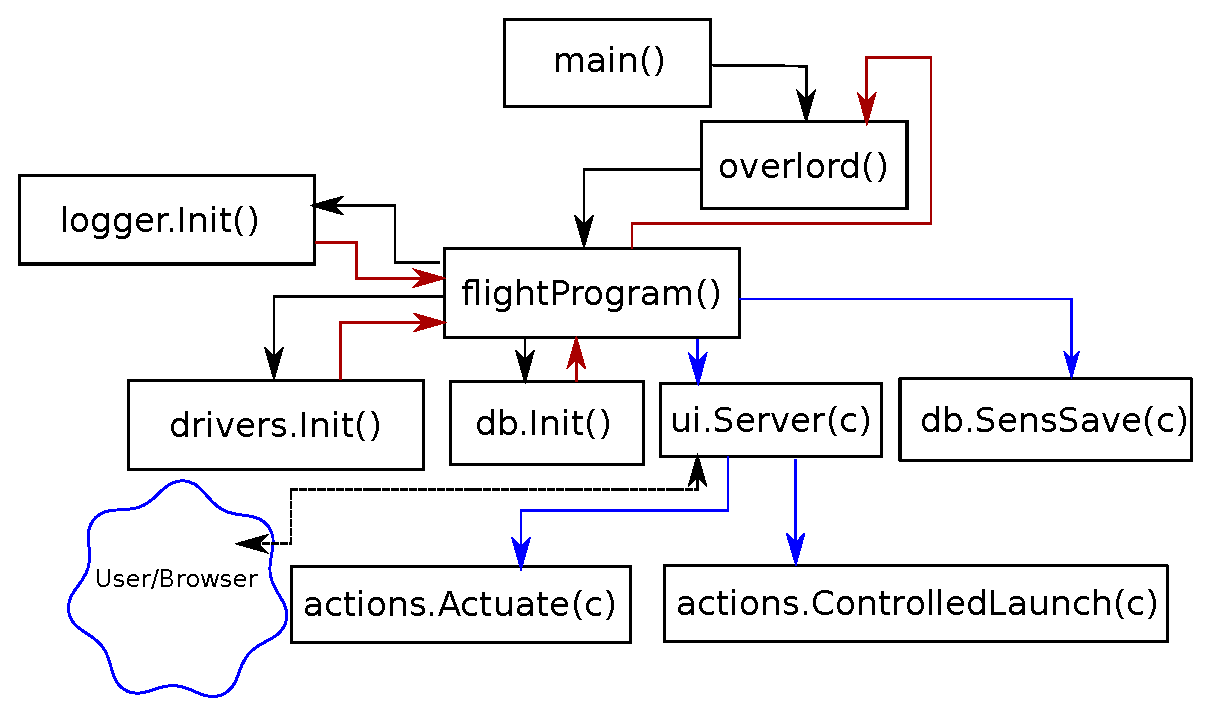
\includegraphics[width=0.7\textwidth]{fig/cfg_flightprogram.eps}
    \caption{Gráfico de flujo de control (CFG) del programa de vuelo. Las lineas de flujo azules son corrutinas independientes al programa principal. Las lineas negras son flujo del programa principal. Las lineas rojas son flujo del programa principal al encontrar un error.}
    \label{fig:flightProgram}
\end{figure}

Se ilustra el flujo de control a grandes rasgos usando un CFG en la figura \ref{fig:flightProgram}. El programa principal corrió la rutina \texttt{overlord} que a su vez comandó \texttt{flightProgram} y esperó que esta devuelva control a \texttt{overlord}. El propósito de \texttt{overlord} fue guardar el estado del vehículo y ante una falla irrecuperable en \texttt{flightProgram}, terminar con todas las corrutinas generadas por \texttt{flightProgram} y sus afiliadas y a su vez reiniciar \texttt{flightProgram} nuevamente con el último estado antes de la falla.


\subsection{Interfaz con hardware}

Como se mencionó anteriormente, la computadora elegida tiene varios puertos que sirviern como interfases con periféricos, entre ellos 

\begin{itemize}
    \item ADC (sensores)
    \item Generadores de PWM (para actuadores)
    \item Blinkenlights
\end{itemize}

Para la interacción del software con el hardware se usó la librería \href{https://periph.io}{periph.io}. Esta librería permitió la interacción a través de los puertos de comunicación de la Raspberry Pi. Los drivers para los periféricos fueron programados según la información dada en las datasheet.


\subsection{Implementación}

Al momento de escribir el presente informe el programa de vuelo tuvo 3540 líneas de lógica, de las cuales 1680 correspondieron a los drivers de control de periféricos. Se logró controlar la actuación de hasta 12 señales PWM y en simultaneo leer 16 señales de telemetría y guardar a archivo en una tarjeta SD a 1200 muestras por segundo (cada canal). 1060 líneas de código fueron dedicadas a la interfaz de usuario para facilitar el control del vehículo desde un browser, como por ejemplo Firefox.

\subsection{Debugging}

En junio 2021 se halló un bug en el software. Al cabo de cierto tiempo entraba en un estado degenerado el sistema donde no respondía a inputs de usuario ni a señales del sistema operativo. Debido a los periféricos usados la última señal mandada al actuador se quedaba fija y era imposible retornar el sistema a un estado seguro sin terminar el programa forzosamente y reiniciarlo. 

Se sospechaba que el bug era causa de una falla en el kernel de Linux para computadoras ARM o corrupción de memoria causada por el garbage collector de Go. Debido a la configuración de la computadora y las herramientas disponibles para Go era dificil debuggear. El debugger nativo de Go (Delve) no funcionaba aún en procesadores ARM de 32 bits y el detector de carreras de Go tampoco estaba disponible para procesadores ARM. Se pasó 6 meses investigando intermitentemente y hablando con expertos en software y hardware.

En enero 2022 se encontró el mismo comportamiento observado durante el bug mientras se desarrollaba un proyecto no asociado a este trabajo. En este software el estado degenerado era causado por una condición de carrera, específicamente era el caso de una \gls{datarace}. Con este conocimiento se modificó el programa de vuelo para que pueda correr en un entorno de computadora desktop. Para lograr esto se programó un mock de la escritura I2C que fue facilitado por el uso de \textit{interfaces} en Go. Esta modificación permitió al detector de carreras de Go encontrar condiciones de carrera en el programa de vuelo. Se encontraron y se arreglaron 2 condiciones de carreras causadas por error de programador debido al uso equivocado de mutexes.

Aún así el error persistía y el programa seguía encontrandosé en el estado degenerado. Se optó por reescribir el programa de cero y aplicando patrones de diseño más estrictos y seguros. Al cabo de un mes se había reescrito el programa de vuelo de la empresa y el bug no volvió a resurgir en el desarollo. Esto se puede deber a que se redujo el uso de librerias de terceros y la cantidad de líneas de código totales bajó de 700.000 a tan solo 30.000, incluyendo dependencias de terceros3. Excluyendo las liberías de terceros, la base de código era de tan solo 2100 líneas e incluía el frontend (interfaz con el usuario).

